\providecommand{\methoddetail}[1]{}
\providecommand{\methodsep}{}
\chapter{Related work on pruning: Structured Methods}
\label{chap:related_work_pruning_structured}


\section{Introduction}
While Chapter \ref{chap:related_work_pruning_unstructured} explored methods that remove individual weights or apply heterogeneous sparsity profiles, those approaches often rely on specialized sparse-execution hardware to achieve real-world latency reductions. This chapter shifts focus to the other side of our taxonomy: Structured Pruning.

Instead of scattering zeros throughout a weight matrix, structured pruning removes entire executable units such as attention heads, feed-forward channels, or complete Transformer layers. By excising these structural blocks, the resulting compressed model remains a standard, albeit smaller, dense neural network. This allows it to be accelerated on any standard hardware using highly optimized dense matrix multiplications, achieving immediate out-of-the-box speedups.

However, removing entire structural units is highly destructive to the model's forward pass, making the criteria for removal significantly more complex than unstructured weight magnitude. Based on the taxonomy established previously, this chapter reviews four prominent structured pruning methodologies: LLM-Pruner, CoFi, Fast Post-Training Pruning (Fast PTPF), and ZipLM. These methods represent the state-of-the-art in overcoming the destructive nature of structured removals, utilizing dependency graphs, learnable masks, and second-order optimization.

\section{Gradient-Based Methods}

The first order term of the Taylor expansion (Equation~\eqref{eq:taylor}) retains a value that is a product of the gradient and the weight value. The criterion thus becomes sensitive to the direction of loss change as well as the weight magnitude. The methods in this section utilize precisely this first order signal, however instead of single values it utilizes grouped structure, for example heads, channels and blocks.

Structured pruning replaces individual-weight saliency with group-level importance, because the natural units in a Transformer, namely attention heads, FFN channels, and entire layers, are coupled through residual pathways and shared projection matrices. Removing one head, for example, requires deleting consistent slices from $W_Q$, $W_K$, $W_V$, and $W_O$ together; removing an FFN channel removes coordinated rows and columns from the two projection matrices. Any pruning criterion applied at this level must therefore identify groups that can be removed as a unit without breaking the forward pass \cite{michel2022not,kurtic2022optimal}.

\paragraph{LLM-Pruner.}
LLM-Pruner \cite{ma2023llmpruner} addresses the dependency problem explicitly by constructing a graph over the neurons of the network. For neurons $N_i$ and $N_j$ with input set $\mathrm{In}(N)$ and output set $\mathrm{Out}(N)$, the graph encodes two rules:
\begin{align}
	N_j \in \mathrm{Out}(N_i) \wedge \deg^{-}(N_j)=1 &\implies N_j \text{ depends on } N_i, \label{eq:dep1}\\
	N_i \in \mathrm{In}(N_j) \wedge \deg^{+}(N_i)=1 &\implies N_i \text{ depends on } N_j. \label{eq:dep2}
\end{align}
Here $\deg^{-}(N_j)$ is the in-degree of $N_j$ (number of neurons feeding into it) and $\deg^{+}(N_i)$ is the out-degree of $N_i$. The transitive closure of these rules groups all coupled parameters into a single dependency group $\mathcal{G} = \{W_i\}_{i=1}^M$, which is the minimal unit that can be consistently removed.

Once groups are defined, each is scored using a first-order Taylor approximation of the loss increase over a small calibration set $\mathcal{D}$. The importance of a structure tensor $W_i$ is estimated as
\begin{equation}
	I_{W_i}
	\approx
	\left|
	\frac{\partial \mathcal{L}^{\top}(\mathcal{D})}{\partial W_i}W_i
	-\frac{1}{2}W_i^{\top}HW_i
	\right|,
	\label{eq:taylor-vector}
\end{equation}
where $H$ is the local Hessian. The first-order gradient is retained alongside the Hessian term because the calibration set is only a proxy for the pretraining distribution; discarding it would introduce bias. An element-wise variant replaces $H$ with a Fisher-diagonal approximation. Individual tensor scores within a group are aggregated by sum, product, max, or last-only operators, and groups with the lowest aggregate score are removed first.

LLM-Pruner sits between a post-training and a recovery regime: scoring is post-training and requires no gradient propagation through the full model, but the pruned network is then passed through a LoRA recovery stage in line with the iterative recovery approach of Section~\ref{subsec:iterative_pruning}. LoRA adapters \cite{hu2021lora} are inserted into all linear modules and fine-tuned for two epochs over roughly 50K samples. The low-rank factors are then merged back into the weight matrices, leaving no adapter overhead at inference time. The full scoring stage requires only 10 short calibration sequences, making the preprocessing cost modest relative to the recovery phase.

\methodsep

\paragraph{CoFi.}
CoFi \cite{xia2022structured} is the main structured-pruning example of the learnable-mask criteria introduced in Section~\ref{subsec:learnable_adaptive_criteria}. It places binary masks on attention blocks, heads, FFN blocks, intermediate channels, and the shared hidden dimension, then optimises these masks jointly with the task loss:
\begin{align}
	\mathrm{MHA}(X) &= z_{\mathrm{MHA}} \sum_{i=1}^{N_h} z_{\mathrm{head}}^{(i)} \,\mathrm{Att}\!\left(W_Q^{(i)},W_K^{(i)},W_V^{(i)},W_O^{(i)},X\right), \\
	\mathrm{FFN}(X) &= z_{\mathrm{FFN}}\, \mathrm{gelu}(XW_U)\,\mathrm{diag}(z_{\mathrm{int}})\,W_D,
\end{align}
where $N_h$ is the number of attention heads, $W_Q^{(i)}, W_K^{(i)}, W_V^{(i)}, W_O^{(i)}$ are the query, key, value, and output projection matrices of head $i$, and $W_U$, $W_D$ are the up- and down-projection matrices of the FFN. Each mask variable $z$ is relaxed to a continuous value during training using the hard-concrete distribution for $L_0$ regularisation, which allows gradients to flow through the mask. The training objective combines task loss with a distillation term and a Lagrangian sparsity constraint:
\begin{equation}
	\mathcal{L}_{\mathrm{prune}}
	=
	\mathcal{L}_{\mathrm{task}}
	+
	\mathcal{L}_{\mathrm{distil}}
	+
	\lambda_1(\hat s - s_0)
	+
	\lambda_2(\hat s - s_0)^2,
\end{equation}
where $s_0$ is the sparsity target and $\hat{s}$ is the expected sparsity under the current mask distribution. Because the masks at different granularities interact, CoFi can discover structured subnetworks that a simple per-group ranking would miss.

\methoddetail{Algorithm Overview}
CoFi is a training-time iterative method in the sense of Section~\ref{subsec:iterative_pruning} where mask decisions and weight updates are interleaved throughout training. A warm-up phase first stabilizes the model weights before mask learning begins, with the sparsity constraint applied softly. The main phase then jointly optimises masks and weights under the Lagrangian objective, progressively tightening the sparsity target toward $s_0$ over training. Once the target is reached, each continuous mask variable is thresholded against zero to produce a binary decision, and a final fine-tuning pass is run on the surviving subnetwork. Because masks at all granularities are trained simultaneously.

Gradient-based structured pruning improves the consistency of the removed units, but the score still depends on a local approximation of how removal affects the loss. When pruning becomes more aggressive, interactions among remaining and removed weights become more important. This leads to second-order methods, which use curvature information or local reconstruction objectives to compensate for the error introduced by pruning.



\section{Second-Order Structured Methods}

The second-order term of the Taylor expansion (Equation~\eqref{eq:taylor}) captures the curvature of the loss around the current weights. Retaining this term allows the
pruning criterion to account for how much a removal actually shifts the loss given the local geometry of the loss landscape. As discussed in Section~\ref{subsec:second_order_criteria}, this leads to the OBS framework, where the optimal weight correction after a removal is derived from the inverse Hessian. The methods in this section apply that same principle the scale of modern LLMs, recovering tractability by restricting the Hessian computation to individual layers or column blocks.

\subsection{Optimal Brain Compression Formulation}

For a layer with weight matrix $\mathbf{W} \in \mathbb{R}^{d_{\text{out}} \times d_{\text{in}}}$ and calibration activations $\mathbf{X} \in \mathbb{R}^{d_{\text{in}} \times n}$, the layer-wise sparse reconstruction problem is
\begin{equation}
	\min_{\mathbf{W}^{\text{sparse}}}
	\|\mathbf{W}\mathbf{X} - \mathbf{W}^{\text{sparse}}\mathbf{X}\|_F^2
	\quad \text{s.t.} \quad
	\|\mathbf{W}^{\text{sparse}}\|_0 \leq (1-p)\, d_{\text{out}} d_{\text{in}},
\end{equation}
where $\|\cdot\|_F$ is the Frobenius norm, $\|\cdot\|_0$ counts the number of nonzero entries, and $p \in (0,1)$ is the target sparsity ratio. Using the empirical Hessian proxy $\mathbf{H} = \mathbf{X}\mathbf{X}^T / n$, this becomes a curvature-aware reconstruction problem whose solution depends on $\mathbf{H}^{-1}$ to redistribute pruning error across remaining weights. The methods that follow differ in how they instantiate this objective: SparseGPT removes one scalar weight at a time, MRP removes an entire N:M group jointly, Fisher-based pruning applies curvature scoring to structured masks, and ZipLM extends the same principle to executable Transformer structures under runtime constraints.

\subsection{Single-Weight Iterative Removal (SparseGPT)}

SparseGPT \cite{frantar2023sparsegpt} greedily prunes one weight at a time while applying compensation updates to remaining weights in the current block. This can be read as a blockwise version of the OBS correction introduced in Section~\ref{subsec:obd_obs} and formalised for large linear layers in Section~\ref{subsec:second_order_criteria}. Its local objective at iteration $t$ is
\begin{equation}\label{eq:srp}
	\min_{\delta w} \frac{1}{2}\delta w^T H \delta w
	\quad\text{s.t.}\quad
	(w+\delta w)\cdot e_t = 0,
\end{equation}
where $e_t$ is the one-hot selector for the pruned weight.

\methoddetail{Algorithm Overview}
SparseGPT is a post-training one-shot method in the regime of Section~\ref{sec:post_training_pruning}: pruning and compensation are applied in a single forward pass over the layers without any subsequent gradient-based recovery. It processes the weight matrix in column blocks of size $B$. For each block, it first constructs the regularized inverse Hessian $(XX^T + \lambda I)^{-1}$. Within each block, it iteratively identifies the weight with minimum local second-order loss, sets it to zero, then updates the remaining weights in that block using the corresponding column of $\mathbf{H}^{-1}$. After processing a block, lazy batch updates are applied to adjacent blocks. The method scales as $O(d_{\text{in}}^2 d_{\text{out}} + d_{\text{in}}^3/B)$ per layer, with a calibration budget of approximately 128 samples.

It is more instructive to understand SparseGPT as a weight-level, Hessian-compensated method for pruning: each decision to prune weights is made locally, and weights are updated to make the layer output's deviation as minimal as possible \cite{frantar2023sparsegpt}. It is through this same lens that SparseGPT's modification for semi-structured N:M sparsity can be understood, where the compensation method is kept and mask selection is constrained to local groups. If the block size is set to $B_s = M$, and from each group of $M$ weights the $N$ weights with the smallest OBS reconstruction score are selected for removal, the compensation becomes more localized to a block instead of applying it for the entire layer and that is to save computation. Within that block, however, weights are still selected and compensated one at a time, so the compensation at each step does not account for the interactions among the other weights being simultaneously removed from the same group, which is the gap MRP directly addresses.

\methodsep

\subsection{Joint Optimization for Multi-Weight Removal (MRP)}

The MRP framework \cite{zhao2024pruning} generalizes second-order pruning to N:M groups. For a vectorized weight block $w$ and binary pruning mask $M$, where $M_i=1$ indicates that weight $i$ is pruned, the objective minimizes the second-order loss increase for the full group:
\begin{equation}\label{eq:ptp}
	\min_{\delta w} \frac{1}{2}\delta w^T H \delta w + g^T \delta w
	\quad\text{s.t.}\quad
	(w+\delta w)\odot M = 0,
\end{equation}
where $g$ is the gradient of the loss with respect to $w$, and $\odot$ denotes elementwise multiplication. Solving the group jointly yields a compensation update for the retained weights:
\begin{equation}
	\delta w^\star = -H_{\bar{M}\bar{M}}^{-1}(g_{\bar{M}} + H_{\bar{M}M}w_M),
\end{equation}
where $M$ denotes pruned indices, $\bar{M}$ retained indices, and $w_M$ the weight values at the pruned coordinates. This expression makes the role of the block Hessian explicit: in N:M pruning, the removed weights are not independent decisions, so compensation must be computed for the group.

\methoddetail{Algorithm Overview}
MRP is a post-training one-shot method in the regime of Section~\ref{sec:post_training_pruning}: no gradient updates or recovery training are applied after pruning. It operates layer by layer. For each layer, the block Hessian is estimated from calibration activations. The weight tensor is partitioned into non-overlapping groups of $M$ consecutive weights. For each group, the joint second-order problem is solved: the mask selecting the $M-N$ weights with the highest reconstruction cost is identified, and the compensation update $\delta w^\star$ is applied to the retained $N$ weights before the next group is processed. Because the group is treated as a unit or a group, the method correctly accounts for interactions among simultaneously pruned coordinates within the block.

Figure~\ref{fig:hessian_compensation} illustrates this difference. SparseGPT compensates after removing one scalar weight, whereas MRP compensates after removing a constrained local group. The figure is therefore used to distinguish scalar second-order correction from group-level second-order correction.

\begin{figure}[H]
\centering
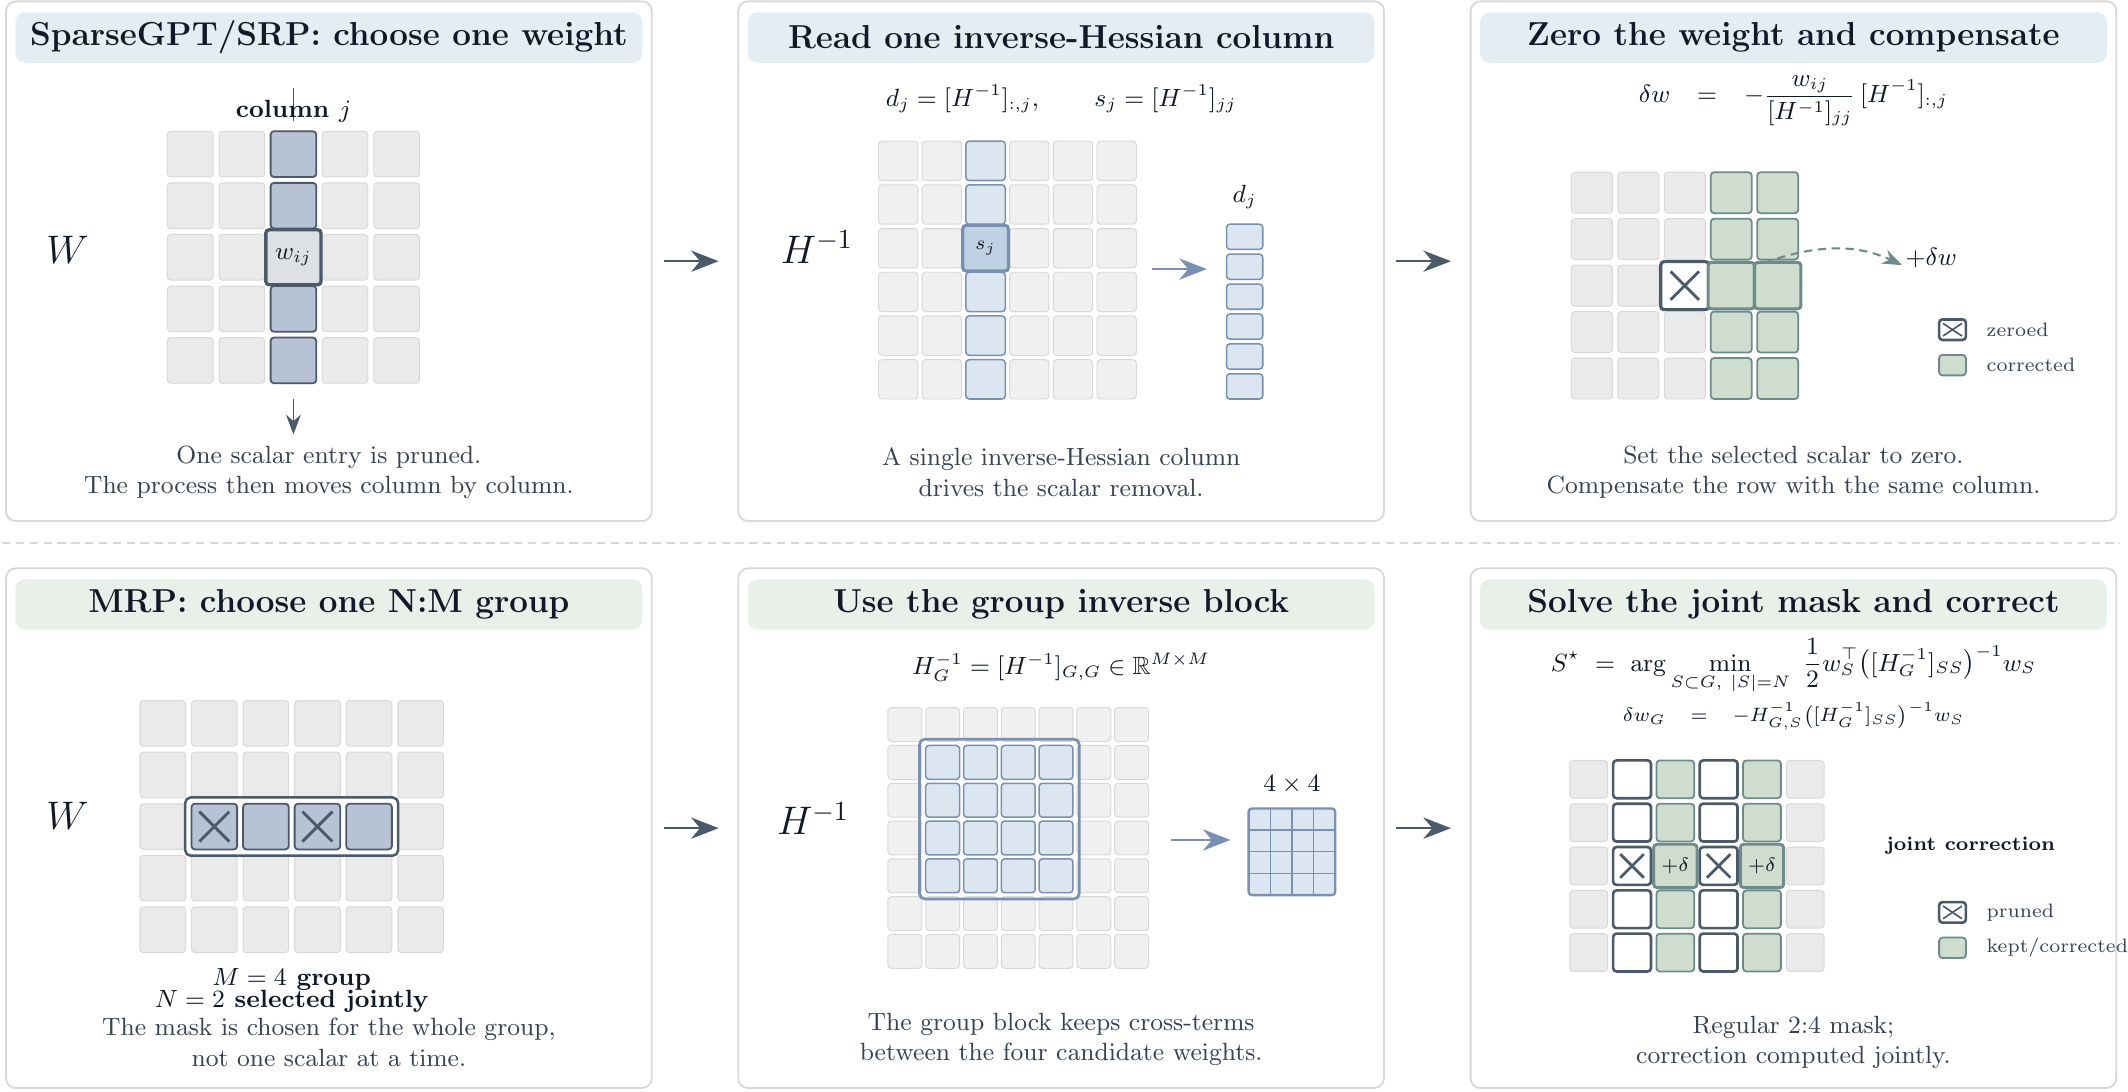
\includegraphics[width=0.8\linewidth]{figures/compression/sparsegpt_mrp_compensation.png}
\caption[Second-order compensation strategies for unstructured and semi-structured pruning.]{Second-order compensation strategies for unstructured and semi-structured pruning.}
\label{fig:hessian_compensation}
\end{figure}

\methodsep

\subsection{Fisher-Based Post-Training Structured Pruning}

The post-training framework of Kwon et al. \cite{kwon2022fast} applies second-order structured pruning without end-to-end post-pruning weight optimization. Binary masks over attention heads and FFN filters are found by solving
\begin{equation}
	\arg\min_{\mathbf{m}} \mathcal{L}(\mathbf{m})
	\quad \text{s.t.} \quad
	\mathrm{Cost}(\mathbf{m}) \leq C,
\end{equation}
where $\mathrm{Cost}$ is either a FLOPs or measured latency budget. Expanding around the dense mask and applying a diagonal Fisher approximation reduces the search to selecting units with the smallest diagonal Fisher scores subject to the cost constraint. For latency-constrained pruning, a piecewise-linear lookup table replaces the analytical cost model to incorporate real device behavior:
\begin{equation}
	\mathrm{LAT}(\mathbf{m}_{\ell}) =
	\begin{cases}
		0, & \|\mathbf{m}_{\ell}\|_0 = 0, \\
		c, & 0 < \|\mathbf{m}_{\ell}\|_0 \leq T, \\
		a(\|\mathbf{m}_{\ell}\|_0 - T) + c, & \|\mathbf{m}_{\ell}\|_0 > T,
	\end{cases}
\end{equation}
Where $c$ represents the base latency for any non-empty layer settings, $T$ denotes the structural threshold below which the latency remains relatively constant, and $a$ is the slope describing how measured latency increases beyond $T$. The lookup table is accessed when searching for the mask to get an estimate for the latency of each pruned MHA or FFN layer on the target device, enabling the selection of a mask that fulfills a measured latency budget.

\methoddetail{Algorithm Overview}
The method proceeds in four steps: (1) diagonal Fisher scores are computed for head and FFN-filter masks on a small calibration set (2K training examples); (2) a FLOPs- or latency-constrained mask search is solved under the diagonal Fisher objective; (3) a block-diagonal Fisher refinement is applied layer by layer to recover interactions ignored by the diagonal approximation; (4) surviving mask values are tuned by layer-wise linear least-squares reconstruction. Because only mask values are updated, the method avoids end-to-end weight retraining. The paper reports pruning times of 39 seconds on GLUE and 135 seconds on SQuAD, compared to 33 hours for CoFi on MNLI.

\methodsep

\subsection{Inference-Aware Structured Second-Order Pruning (ZipLM)}

ZipLM\cite{kurtic2023ziplm} extends the OBS-style reconstruction objective from individual weights to executable Transformer structures. The pruned objects are attention heads, FFN intermediate channels, and, at the coarser level, entire residual modules such as the attention block or the FFN block. For a candidate structure $S$ with column mask $\mathbf{M}_S$, the removal score is
\begin{equation}
	\arg\min_S
	\sum_{i=1}^{d_{\text{row}}}
	\mathbf{W}_{i,\mathbf{M}_S}
	\left(\left(\mathbf{H}^{-1}\right)_{\mathbf{M}_S,\mathbf{M}_S}\right)^{-1}
	\mathbf{W}_{i,\mathbf{M}_S}^{T},
\end{equation}
where $d_{\text{row}}$ is the output dimension of the weight matrix and the sum aggregates the reconstruction cost across all output rows. After removing a structure, the exact compensation and Hessian update are applied through block Gaussian elimination, so that all subsequent saliency scores remain consistent with the already-pruned state.

\methoddetail{Inference-Aware Search}
ZipLM adds a device-level objective on top of the local second-order scoring. It benchmarks attention and FFN configurations on the target hardware and stores measured runtimes in a lookup table. The global search then minimizes layer-wise structural sensitivity subject to a real speed constraint $\sum_\ell \tau_{\ell,s_\ell} \leq T_{\text{target}}$.

\methoddetail{Algorithm Overview}
ZipLM follows an iterative pruning-and-recovery regime in the sense of Section~\ref{subsec:iterative_pruning}: pruning steps are interleaved with fine-tuning rounds. It operates in two phases (see Figure~\ref{fig:ziplm_pipeline}). In the global phase, attention-head and FFN configurations are benchmarked on the target environment and a layer-wise sparsity profile satisfying the speedup requirement is selected. In the local phase, each selected layer is compressed by iteratively scoring candidate structures with the structured saliency metric, applying the optimal weight compensation, and updating the inverse Hessian by block Gaussian elimination. Recovery follows a gradual prune-and-fine-tune schedule with combined task, logit, and token-level distillation losses, at a cost of 8--10 fine-tuning epochs per pruning step.

\begin{figure}[H]
	\centering
	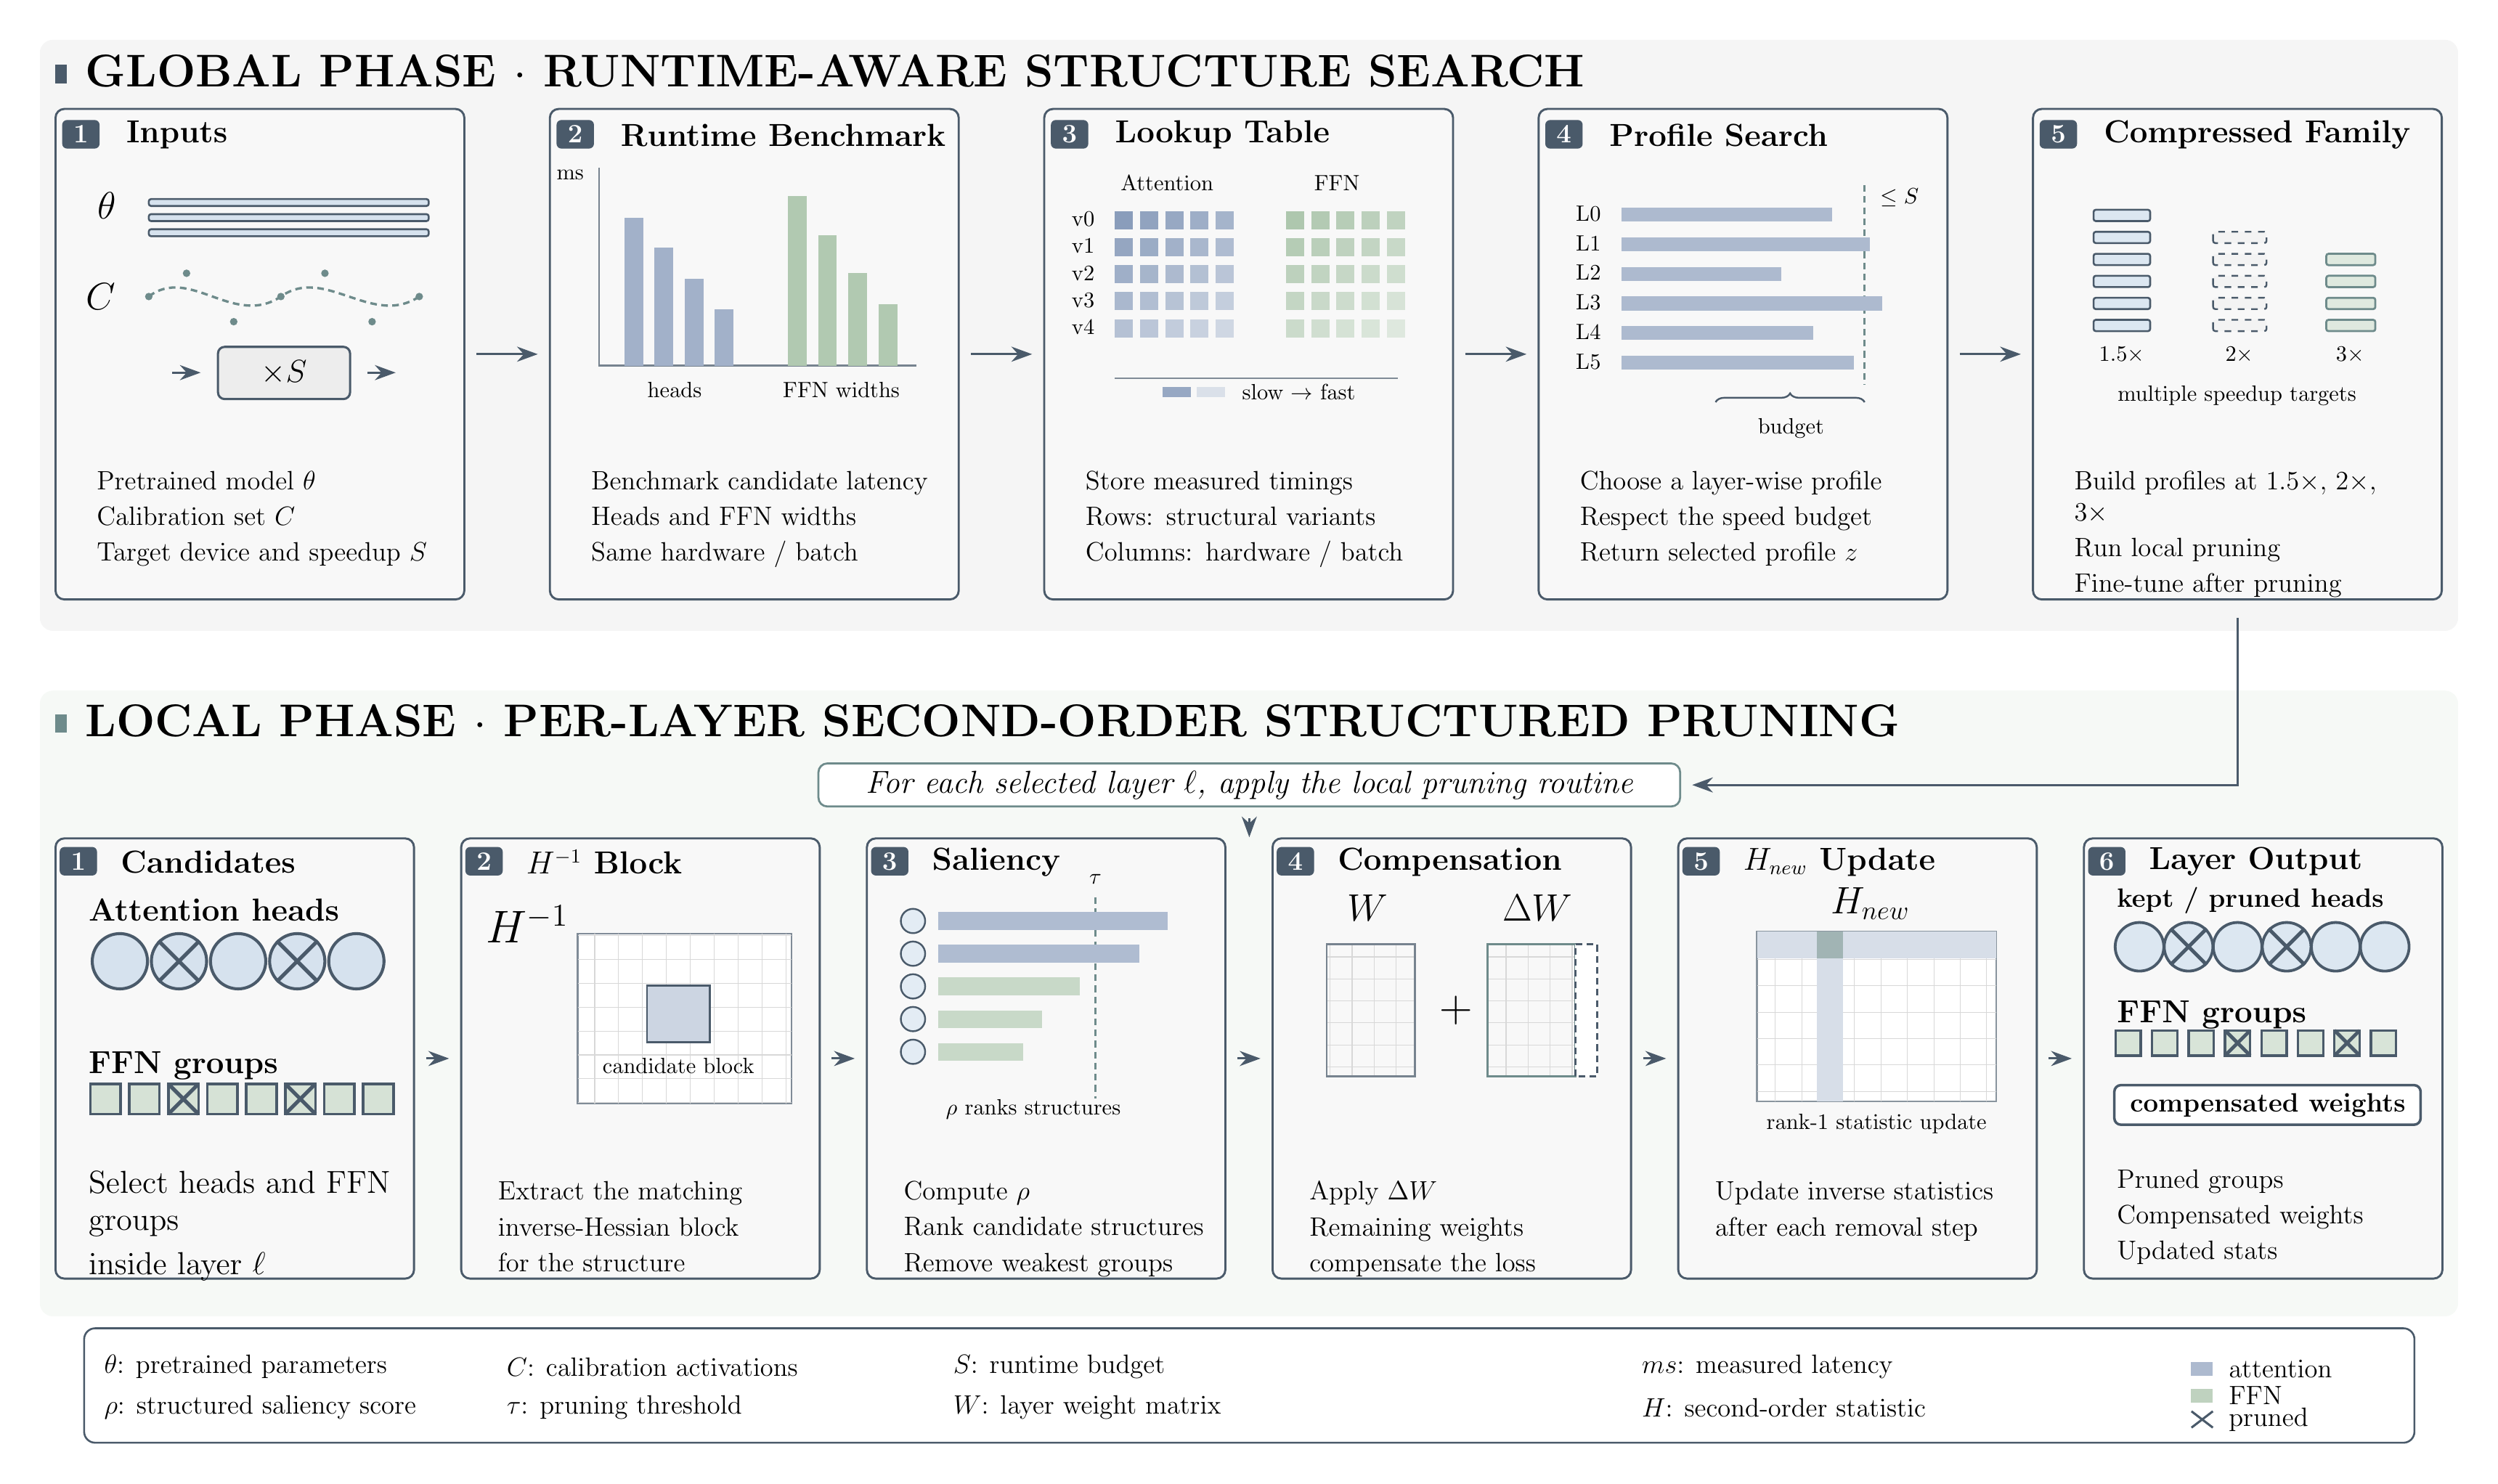
\includegraphics[width=0.96\textwidth]{figures/compression/ziplm_diagram.png}
	\caption[ZipLM pipeline.]{ZipLM pipeline. The global phase benchmarks attention-head and FFN configurations and searches for layer-wise sparsity profiles satisfying the required speedup. The local phase applies second-order structured pruning through inverse-Hessian scoring, compensation updates, and iterative Hessian refinement.}
	\label{fig:ziplm_pipeline}
\end{figure}

Second-order methods reduce local reconstruction error, but they do not fully resolve the allocation problem across the whole model. A method may know how to remove a head or channel with limited local damage and still not know how many heads or FFN channels should remain in each layer under a global budget. This is the point at which search-based methods become relevant.
\section{Conclusion}
This chapter examined structured pruning as a mechanism for generating hardware-agnostic, dense-shape acceleration. By reviewing LLM-Pruner, CoFi, Fast PTPF, and ZipLM, we illustrated how the pruning objective must adapt when removing highly coupled components like attention heads and feed-forward channels. Because structural removals are highly destructive, these methods rely on sophisticated techniques to preserve accuracy, ranging from dependency mapping to joint mask optimization and second-order Hessian compensations.

However, evaluating these methods in isolation only tells half the story. To understand the true state of Transformer compression, we must compare the structured methods discussed in this chapter with the unstructured and heterogeneous methods from Chapter 4. Therefore, the following chapter will provide a comprehensive cross-regime empirical comparison, identify the critical limitations in current evaluation protocols, and formally define the unresolved ``allocation problem'' that motivates the contribution of this thesis.



\chapter{Synthesis, Empirical Comparison, and Limitations}
\label{chap:pruning_comparison}
\section{Introduction}
The previous two chapters surveyed Transformer pruning through unstructured/heterogeneous methods (Chapter 4) and structured methods (Chapter 5). These methods optimize different units, rely on different recovery pipelines, and target different deployment metrics, so their results cannot be reduced to a single compression table. The comparison in this chapter focuses on what the evidence actually supports: where pruning remains accurate, where recovery dominates the result, and where local scoring fails to determine a strong global configuration.


\section{Empirical Comparison}
\label{subsec:empirical_comparison}

The empirical results are grouped by pruning regime because each regime reports a different kind of outcome. Unstructured and N:M methods mainly report perplexity under weight sparsity, structured methods report task accuracy or speedup after architectural removal, and search-based methods report complete pruning configurations under budget constraints.

\subsection{Unstructured and Semi-Structured Results}

Table~\ref{tab:unsupported_comparison} reports representative low, medium, and large model settings. The unstructured rows compare magnitude pruning, SparseGPT, and Wanda at 50\% sparsity, and the 2:4 rows show the semi-structured setting that motivates group-aware compensation such as MRP.

\begin{table}[H]
	\centering
	\caption[Representative unstructured and semi-structured pruning results on WikiText perplexity.]{Representative unstructured and semi-structured pruning results on WikiText perplexity. PPL denotes perplexity; lower is better.}
	\label{tab:unsupported_comparison}
	\begin{tabular}{@{}llcccc@{}}
		\toprule
		\textbf{Model} & \textbf{Setting} & \textbf{Dense PPL} & \textbf{Magnitude PPL} & \textbf{SparseGPT PPL} & \textbf{Wanda PPL} \\
		\midrule
		LLaMA-7B  & 50\% unstructured & 5.68 & 17.29 & 7.22 & 7.26 \\
		LLaMA-30B & 50\% unstructured & 4.77 & 7.54  & 5.31 & 5.24 \\
		LLaMA-65B & 50\% unstructured & 3.56 & 5.90  & 4.57 & 4.57 \\
		\midrule
		OPT-13B   & 50\% unstructured & 10.13 & $1.2{\times}10^4$ & 11.17 & -- \\
		OPT-175B  & 50\% unstructured & 8.35  & $4.3{\times}10^4$ & 8.21  & -- \\
		\midrule
		OPT-13B   & 2:4 semi-structured & 10.13 & -- & 12.96 & -- \\
		OPT-66B   & 2:4 semi-structured & 9.34  & -- & 10.09 & -- \\
		OPT-175B  & 2:4 semi-structured & 8.35  & -- & 8.74  & -- \\
		\bottomrule
	\end{tabular}
\end{table}

The results show that pure magnitude pruning can fail badly at 50\% sparsity, especially on OPT models, whereas activation-aware and second-order criteria preserve perplexity much more effectively. The 2:4 rows also show that semi-structured pruning is not just unstructured pruning with a different mask shape: the local group constraint changes the compensation problem and motivates methods such as MRP.

\subsection{Structured Pruning Results}

Table~\ref{tab:structured_summary} summarizes representative structured-pruning results across compression and speedup regimes. The table keeps the evaluation suite explicit: CoFi is reported on GLUE tasks and SQuADv1, Fast PTPF reports GLUE/SQuAD results, and ZipLM reports GLUE-style classification tasks and SQuADv1.

\begin{table}[H]
	\centering
	\caption[Representative structured Transformer pruning results across recovery regimes.]{Representative structured Transformer pruning results across recovery regimes. GLUE denotes the General Language Understanding Evaluation benchmark, SQuADv1 denotes Stanford Question Answering Dataset version 1.1, acc. denotes accuracy, and F1 denotes question-answering F1 score.}
	\label{tab:structured_summary}
	\begin{tabular}{@{}llp{4.4cm}p{4.7cm}@{}}
		\toprule
		\textbf{Method} & \textbf{Model} & \textbf{Setting} & \textbf{Key result} \\
		\midrule
		LLM-Pruner \cite{ma2023llmpruner}
		  & LLaMA-7B & 20\% prune ratio & 94.97\% zero-shot accuracy retention after LoRA recovery \\
		  & LLaMA-7B & 50\% prune ratio & 77.4\% zero-shot accuracy retention after LoRA recovery \\
		\midrule
		CoFi \cite{xia2022structured}
		  & BERT Base & GLUE/MNLI, $\approx 12{\times}$ speedup & 80.6 acc.; TinyBERT$_4$ reports 78.8 at similar speedup \\
		  & BERT Base & SQuADv1, $\approx 8.7{\times}$ speedup & 82.6 F1, matching TinyBERT$_4$ at comparable speedup \\
		\midrule
		Fast PTPF \cite{kwon2022fast}
		  & BERT Base & GLUE and SQuADv1, FLOPs-constrained pruning & 60--70\% FLOPs with $\leq 1\%$ accuracy/F1 drop \\
		  & BERT Base & GLUE and SQuADv1, latency-constrained pruning on V100 & $1.34{\times}$--$1.47{\times}$ geometric-mean speedup depending on batch size \\
		\midrule
		ZipLM \cite{kurtic2023ziplm}
		  & BERT Base & GLUE/QNLI and MNLI, $2{\times}$ speedup & 91.4 / 84.8 acc.; essentially dense-level performance \\
		  & BERT Base & GLUE/QNLI and MNLI, $10{\times}$ speedup & 88.6 / 82.7 acc.; approximately 5M parameters \\
		  & BERT Large & SQuADv1, $10{\times}$ speedup & 89.1 F1 with 20.9M parameters \\
		\bottomrule
	\end{tabular}
\end{table}

These results are closer to deployment because the methods remove executable units, but they still depend heavily on the evaluation and recovery setup. CoFi uses task-specific training, LLM-Pruner depends on LoRA recovery, Fast PTPF is largely post-training, and ZipLM adds device-specific runtime profiling. The numbers therefore show the achievable trade-offs within each protocol, not a clean ranking across methods.

\subsection{Evolutionary and Search-Based Results}

Table~\ref{tab:search_summary} reports representative search-based results for EvoPress and DarwinLM. EvoPress searches over depth-pruning and sparsity-allocation configurations, and DarwinLM uses structured evolutionary pruning with training-aware offspring selection.

\begin{table}[H]
	\centering
	\caption[Representative search-based pruning results]{Representative search-based pruning results. Wiki2 and C4 are perplexity values where lower is better; task average is accuracy where higher is better.}
	\label{tab:search_summary}
	\begin{tabular}{@{}llllccc@{}}
		\toprule
		\textbf{Setting} & \textbf{Model} & \textbf{Budget} & \textbf{Method} & \textbf{Wiki2$\downarrow$} & \textbf{C4$\downarrow$} & \textbf{Task Avg.$\uparrow$} \\
		\midrule
		Depth pruning
		  & Mistral-7B & 25\% & EvoPress & \textbf{8.66} & \textbf{12.04} & -- \\
		  & Mistral-7B & 25\% & ShortGPT & 43.26 & 40.16 & -- \\
		  & Mistral-7B & 25\% & Shortened LLaMA & 14.94 & 19.30 & -- \\
		\midrule
		Depth pruning
		  & Llama-2-7B & 37.5\% & EvoPress & \textbf{17.98} & \textbf{18.91} & -- \\
		  & Llama-2-7B & 37.5\% & ShortGPT & 70.94 & 63.51 & -- \\
		  & Llama-2-7B & 37.5\% & Shortened LLaMA & 35.37 & 26.07 & -- \\
		\midrule
		Unstructured allocation
		  & Mistral-7B & 70\% & EvoPress & \textbf{14.42} & \textbf{16.46} & \textbf{53.8} \\
		  & Mistral-7B & 70\% & OWL & 17.22 & 21.66 & 51.9 \\
		  & Mistral-7B & 70\% & Uniform & 23.08 & 30.03 & 49.9 \\
		\midrule
		Structured search
		  & Llama-2-7B & 2.7B model & DarwinLM & -- & -- & 62.8 after 10B-token post-training \\
		  & Llama-2-7B & 2.7B model & ShearedLLaMA & -- & -- & 62.6 after 50B-token post-training \\
		\bottomrule
	\end{tabular}
\end{table}

The search-based results make the allocation issue explicit. EvoPress improves over local or heuristic allocation when multiple removals interact, and DarwinLM shows that training-aware evolutionary selection can produce strong structured models with less post-training data than a fixed pruning baseline.

\subsection{Cross-Regime Synthesis}

Table~\ref{tab:pruning_empirical_summary} condenses these comparisons into the main implications for pruning-search design.

\begin{table}[H]
	\centering
	\caption{Aggregated interpretation of the empirical pruning evidence by regime.}
	\label{tab:pruning_empirical_summary}
	\begin{tabularx}{\textwidth}{@{}>{\raggedright\arraybackslash}p{2.5cm}>{\raggedright\arraybackslash}p{3.0cm}LL@{}}
		\toprule
		\textbf{Regime} & \textbf{Representative setting} & \textbf{Selected evidence} & \textbf{Reading} \\
		\midrule
		Weight-level unstructured
		& LLaMA-7B, 50\% sparsity
		& Dense PPL 5.68; magnitude 17.29; SparseGPT 7.22; Wanda 7.26.
		& Better saliency preserves perplexity, but the resulting pattern remains unstructured and does not guarantee dense-kernel speedup. \\
		\addlinespace
		Semi-structured N:M
		& OPT-13B, 2:4 sparsity
		& Dense PPL 10.13; SparseGPT-style compensation gives 12.96 under the 2:4 constraint.
		& N:M sparsity needs group-aware compensation, which motivates MRP-style joint treatment of simultaneously removed weights. \\
		\addlinespace
		Structured LLM pruning
		& LLM-Pruner on LLaMA-7B
		& 20\% prune ratio retains 98.6\% zero-shot accuracy after LoRA recovery; 50\% retains 83.6\%.
		& Dependency-aware pruning keeps the model executable, with final quality strongly tied to recovery. \\
		\addlinespace
		Structured encoder pruning
		& CoFi, Fast PTPF, and ZipLM on BERT
		& CoFi reaches 80.6 MNLI acc. near $12{\times}$ speedup; Fast PTPF keeps 60--70\% FLOPs with $\leq$1\% drop; ZipLM reaches 88.6/82.7 QNLI/MNLI acc. at $10{\times}$ speedup.
		& Structured pruning can produce executable acceleration, with protocols differing in training cost, hardware profiling, and recovery budget. \\
		\addlinespace
		Search-based pruning
		& EvoPress and DarwinLM
		& EvoPress improves depth-pruning and sparsity-allocation baselines; DarwinLM reports 62.8 average accuracy after 10B-token post-training versus 62.6 for ShearedLLaMA after 50B tokens.
		& Configuration search addresses global allocation, and training-aware selection improves structured candidates beyond one-shot scoring. \\
		\bottomrule
	\end{tabularx}
\end{table}


\begingroup
\def\RenderPruningReviewDiscussion{}
% ============================================================
%  Drop-in discussion sections, compile inside your main .tex
%  Requires: amsmath, booktabs, enumitem, hyperref, algorithm,
%            algpseudocode, multirow, tabularx, array, xcolor
% ============================================================

% =============================================================
\ifdefined\RenderPruningReviewDiscussion
\section{Discussion}
\label{sec:discussion}
% =============================================================

The distinction between the two questions has been separated between Chapters~\ref{chap:related_work_pruning_unstructured} and~\ref{chap:related_work_pruning_structured} and in the empirical comparison, Section~\ref{subsec:empirical_comparison}. One question is: for a single unit that is potentially removable, what criterion should be used to rank the units? Here, different magnitude-based, gradient-based, and curvature-based criteria offer varying estimates. The second question is: how is the overall budget of pruning shared among the units in the model? Here, the approaches tend to diverge more substantially, and much of the outstanding debate in the literature is focused on the latter. It will be discussed here, then the empirical data.

\subsection{Local Scoring Versus Global Allocation}
\label{subsec:local_vs_global}

The methods reviewed in this chapter differ in implementation, pruning unit, and recovery cost, but they can all be related to the same underlying objective:
\begin{equation}
  \min_{\mathcal{M} \in \mathcal{F}}\; \Delta\mathcal{L}(\mathcal{M}),
  \label{eq:master}
\end{equation}
where $\mathcal{M}$ denotes a feasible sparsity pattern or structured subnetwork and $\Delta\mathcal{L}$ denotes the loss increase caused by pruning. The difficulty is that $\mathcal{M}$ must satisfy a compression budget while preserving the behaviour of the model.

Another persistent issue with the pruning criteria discussed so far is their evaluation of weights and activations, which can be removed before the final compressed model is fixed. SparseGPT calculates approximate second-order local reconstruction costs of sets of weights \cite{frantar2023sparsegpt}, while Wanda sorts parameters by a product of weight magnitude and input activation norm \cite{sun2023simple}. These methods are successful in finding some locally removable weights but fail to determine the overall distribution of compression under a fixed budget across the layers \cite{hoefler2021sparsity,cheng2024pruningsurvey}. Though one-shot local pruning works well under low compression ratios, high compression rates require more sophisticated iterative and global-allocation-based pruning methods \cite{janusz2025oneshot}. Several of these recent methods implicitly or explicitly address this issue: ZipLM attempts to find explicit local and global correlations between layers, and EvoPress directly searches over the layer-wise compression budgets that minimize the distribution divergence of the output \cite{kurtic2023ziplm,evopress2024}.

\subsection{Limitations of Local Ranking at High Compression}
\label{subsec:inadequacy}

In the analyses above, we can observe one trend across these method families. It appears that local ranking criteria are successful when the compression ratio is relatively small to medium; when the targeted compression ratio becomes higher, the deficiencies of local ranking criteria tend to become apparent \cite{hoefler2021sparsity,sanh2020movement,bai2024sparsellm,janusz2025oneshot}. This pattern is expected from the definition of the pruning problem: local criteria judge removeable units while the ultimate compressed model has not been formed completely.

For Transformer models, structured pruning is naturally expressed as a layer-wise allocation problem over executable units. A pruned Transformer may retain different numbers of attention heads, FFN intermediate dimensions, hidden dimensions, or even complete MHA/FFN modules in different layers \cite{xia2022structured,kurtic2023ziplm,cheng2024pruningsurvey}. Thus, for a model with $L$ layers, $H$ attention heads per layer, and $F$ FFN channels per layer, the retained structure can be represented by an allocation vector
\[
  \mathbf{s} = (h_1, f_1, h_2, f_2, \ldots, h_L, f_L),
\]
subject to a global MAC budget $\Omega$. Recent layer-wise pruning work therefore treats compression as the problem of assigning adaptive sparsity ratios across layers which is just a specific case of non uniform pruning \cite{li2024dsa}.

Local ranking simply assigns each prunable unit a saliency and prunes the lowest ones until the budget is exhausted. it implicitly models global ranking with the assumption that each pruning decision can be made in isolation. EvoPress recognizes this assumption in the domain of depth pruning; block-scoring algorithms use the assumption that error is linear such that each block is thought to contribute equally to the overall compression error \cite{evopress2024}. ZipLM takes the reverse argument, stating that pruning has to capture both within layer local correlations and across layer global correlations \cite{kurtic2023ziplm}.

The compositional structure of the Transformer violates the independence approximation. Each Transformer block comprises the residual-connected attention and feed-forward sublayers and self-attention layers take representations as input which are generated from previous layers \cite{vaswani2017attention}. With regard to pruning, this indicates that any alteration on one layer will bring new input distribution for the following layers. SparseLLM is the first one who precisely identifies the problem by modeling an LLM as a chain of modules, where outputs of a module become the inputs for another, and points out that local layer error reduction only causes non-optimal performance for the global pruning at a high sparsity rate \cite{bai2024sparsellm}.

The same coupling is present for attention and the global budget constraint. Scaled dot-product attention normalizes the query-key score using a softmax, while multi-head attention merges multiple heads which act on the same input layer \cite{vaswani2017attention}. Experimentally, attention heads can have unequal importance, numerous can be dropped, beyond a threshold, attention collapses catastrophically, and different components of the attention function can have differing sensitivity \cite{michel2022not}. In addition, if the MAC budget is fixed, having high capacity in one layer means we must sacrifice capacity elsewhere. Prior works have indicated the necessity of across-layer uneven sparsity under high compression \cite{gale2019state,sanh2020movement,li2024dsa}.

% =============================================================
\section{Empirical Results}
\label{sec:empirical}
% =============================================================

Having argued that allocation is more important than local scoring at high compression, the question is whether the results reflect this. On the whole, they do but only if we treat apples and oranges distinctly. The results on the unstructured model isolate the saliency rule in the absence of weight sparsity and the structured/search based readings bring back the cost of recovery and the budget allocation aspect.

\subsection{Unstructured and Semi-Structured Methods}
\label{subsec:unstructured_results}

The unstructured pruning results allow three clean comparisons across increasing levels of local sophistication: magnitude baseline, Wanda (activation-aware saliency), and SparseGPT (second-order compensation).

The SparseGPT results primarily highlight the instability of pure magnitude pruning at high sparsity. At 50\% sparsity on OPT-13B, magnitude pruning produces a perplexity of $1.2\times10^4$ compared to the dense model's 10.13. This indicates severe representational degradation under weight selection based solely on individual magnitude. SparseGPT reduces the same setting to 11.17, corresponding to a $+1.04$ increase over the dense model.

The comparison between Wanda and SparseGPT on LLaMA models is also instructive. At 50\% sparsity on LLaMA-7B, Wanda achieves 7.26 versus SparseGPT's 7.22, a negligible 0.04 point difference. On LLaMA-13B, Wanda actually outperforms SparseGPT by 0.06 points (6.15 versus 6.21). This apparent paradox reflects two facts. First, the Wanda activation norm $\|x_j\|_2$ is an effective proxy for the weight's contribution to the output, particularly in models with large activation outliers, which LLaMA models exhibit. Second, the calibration set used for Hessian construction in SparseGPT introduces variance that at moderate sparsity levels can offset the theoretical advantage of curvature information. At higher sparsity levels (70\%+), the second-order advantage of SparseGPT becomes more consistent, because local reconstruction errors accumulate and the precise compensation direction matters more.

\subsection{Structured Methods}
\label{subsec:structured_results_discussion}

Both CoFi and ZipLM obtain similar accuracy at similar speedups but employ very different preparation pipeline. CoFi obtains 80.6 on MNLI with about $12\times$ speedups after 20 hours of combined mask and weight optimization, whereas ZipLM gets 81.7 at $35\times$ through scheduled fine-tuning interspersed with structured pruning stages and dedicated hardware benchmarking. Here the accuracies represent the accuracy of the whole pipeline not only the pruning criterion, because the recovery approaches they employ differ greatly and thus the two methods are not directly comparable.

\subsection{Cross-Method Comparison}
\label{subsec:cross_method}

The tables above support two conclusions. At 50\% unstructured sparsity on OPT-13B, magnitude pruning collapses to a perplexity of $1.2\times10^4$ while SparseGPT reaches 11.17 (Table~\ref{tab:unsupported_comparison}), showing that second-order compensation is necessary once individual weight interactions become non-negligible. At 70\% unstructured sparsity on Mistral-7B, EvoPress reaches 14.42 perplexity while uniform allocation reaches 23.08 (Table~\ref{tab:search_summary}), and at 37.5\% depth sparsity on Llama-2-7B, EvoPress gives 17.98 against ShortGPT's 70.94, showing that global allocation search becomes the dominant factor at high compression.

\section{Limitations of the Reviewed Methods}
\label{sec:limitations}

 The observations above suggest genuine differences between the methods. However, most of the disparity observed is can simply be a reflection of how each paper was evaluated. There are three consistent issues which have affected nearly every cross-paper assertion: unequal testing scenarios, disparate recovery budget sizes and sensitivity to a calibration set whose effect is usually not examined.

\subsection{Evaluation Protocol Heterogeneity}
\label{subsec:eval_protocol}

A significant drawback in the pruning literature is the lack of a universal evaluation protocol. Approaches are presented under five, and possibly more, different evaluation schemes. The first reports language model perplexity under fixed nominal sparsity, while the second measures zero-shot task performance accuracy with or without recovery. The third instead reports supervised fine-tuning performance accuracy with or without recovery, whereas the fourth measures actual wall-clock speedup or latency given particular hardware. Finally, the fifth reports FLOPs reduction compared to the dense model.

These five schemes are incommensurable. A method presenting $99\%$ dense accuracy after $2\times$ FLOPs reduction addresses a different evaluation goal compared to another method presenting $1.5\times$ wall-clock speedup at a $<1\%$ accuracy drop. FLOPs is a hardware-agnostic theoretical metric that does not necessarily linearly translate to wall-clock runtime, which depends on memory bandwidth, batch size, and the particular accelerator execution model. Certain sparse execution formats require hardware support, while the simple unstructured masks often do not result in a proportional wall-clock speedup over standard dense kernels.

The fragmentation of evaluation makes it difficult to compare across papers. If a table presents Wanda~\cite{sun2023simple}, CoFi~\cite{xia2022structured}, LLM-Pruner~\cite{ma2023llmpruner}, ZipLM~\cite{kurtic2023ziplm}, and EvoPress~\cite{evopress2024} in the same rows, one implicitly assumes that they all aim to solve the same problem. In reality, each method targets different budgets, recovery schemes, and deployment targets. When summarized without qualification, the methods present a false picture of one single Pareto frontier.

\subsection{Recovery Budget Inconsistency}
\label{subsec:recovery}

Relatedly is the issue of different recovery budgets. It's expected that structured pruning results in a larger loss in accuracy than unstructured pruning for a given sparsity, making the recovery stage particularly important \cite{xu2026lightweight}. The difference in terminology of ``post-training pruning'' versus ``pruning with fine-tuning'' in reality represents a wide range of recovery costs that contribute to reported accuracy. Among the methods in the above literature, Fisher post-training pruning only tunings the masks with zero weight updates and total tuning time about 39 sec. LLM-Pruner tunings using 2.5 hrs of LoRA recovery on 50k examples with rank 8 adapter. ZipLM tunes over 8-10 epochs per pruning steps with the whole model fine-tuning and full distillation. CoFi joint tunes mask and weights in 40 epochs with a task specific teacher model.

An appropriate comparison needs to keep recovery budgets constant. The model of 40 epochs fine-tuning for CoFi should not be compared to LLM-Pruner's 2.5 hrs of LoRA recovery. Given the same budget, the gap would be much smaller. Very few articles performed such fair comparisons, and thus, some accuracy differences we see in the literature should be attributed to the amount of recovery budget.

\subsection{Calibration Set Sensitivity}
\label{subsec:calibration}

All post-training pruning techniques rely on a calibration set in order to compute either saliency scores, Hessian surrogates, or Fisher information matrices. The specific selection of the calibration set results in differences in the resulting pruned model which are usually not explored in a principled way.

For language models, it is a common practice to use 128–2048 examples from a general language corpus like C4 or WikiText. This is a small fraction of the model’s training distribution, and may not be representative of activation statistics used to determine saliency. LLM-Pruner calibrates using 10 short examples, which is dramatically fewer than SparseGPT's 128 examples and may contribute to variance in its Taylor scores, and consequently in its reported zero-shot accuracies across trials. More generally, all methods employing a calibration set make the implicit assumption that a ranking based on calibration examples transfers to the whole evaluation distribution. It has recently been shown that the calibration set is extremely important in post-training pruning, especially for high sparsity rates, and that pruning works better with calibration data that matches the pre-training distribution \cite{ji2025calibration,bandari2024calibration}.{ji2025calibration,bandari2024calibration}.

% =============================================================
\fi
\ifdefined\RenderProposedPruningSearchFramework
\chapter{Proposed Pruning-Search Framework}
\label{sec:design}
\label{chap:proposed_pruning_search_framework}
% =============================================================

\section{Design Philosophy and Motivation}
\label{subsec:design_philosophy}

The design of the proposed framework follows directly from the gaps identified in Sections~\ref{sec:discussion}--\ref{sec:limitations}. The central premise is that structured pruning at moderate-to-high compression rates is a combinatorial optimisation problem over architectural configurations. The main methodological deficiency in the reviewed methods lies in global allocation strategy rather than in local saliency estimation alone. The pruning-search paper addresses this point explicitly by treating head retention, FFN width, and active depth as a joint discrete decision and by organising the search around feasibility, representation fidelity, and diversity preservation.

Three design principles follow from this premise.
z
\medskip\noindent\textbf{Principle 1: The configuration is the primary optimisation object.} The framework treats the allocation vector $\mathcal{C} = (\mathbf{h}, \mathbf{n})$ as the optimisation variable. Every operation is defined on complete configurations rather than on per-unit scores. This allows direct evaluation of the joint effect of all removals and keeps the budget constraint explicit throughout the search.

\medskip\noindent\textbf{Principle 2: The feasible set is explicitly enforced.} Rather than soft-penalising infeasible configurations, the framework enforces the MAC constraint and minimum active-depth requirement through a repair projection that maps every mutated configuration back into $\mathcal{F}$ before fitness evaluation. This guarantees that every evaluation corresponds to a deployable architecture.

\medskip\noindent\textbf{Principle 3: Diversity is as important as fitness.} Because the configuration space contains many local optima that are structurally distant from each other, a search that maximises raw fitness without diversity control will converge to one architectural type and miss better solutions elsewhere. The framework therefore maintains diversity explicitly through shared-fitness selection, MAP-Elites archiving, and Pareto preservation.

\section{Configuration Space Formalisation}
\label{subsec:config_space}

The pruning-search paper formalises the search variable as a joint head-and-neuron configuration. For a Transformer with $L$ layers and $H$ heads per layer, the candidate is
\begin{equation}
  \mathcal{C} = (\mathbf{h}, \mathbf{n}), \qquad
  \mathbf{h} \in \{0,1\}^{L \times H}, \quad
  \mathbf{n} \in \beta \mathbb{Z}_{\ge 0}^{L},
  \label{eq:design_candidate}
\end{equation}
where $h_{\ell,k}=1$ indicates that head $k$ of layer $\ell$ is retained and $n_\ell$ is the retained FFN width in multiples of a hardware-aligned block size $\beta$.

Let $S$ denote the sequence length, $d$ the hidden dimension, and $d_h=d/H$ the head dimension. The paper uses a direct MAC accounting model in which one retained head contributes
\begin{equation}
  c_h = 4Sd_hd,
  \qquad
  c_n = 2Sd
  \label{eq:design_mac_unit}
\end{equation}
per retained FFN neuron block. The total cost is therefore
\begin{equation}
  \mathrm{MAC}(\mathcal{C})
  = \sum_{\ell=1}^{L}
  \Bigl(
    \sum_{k=1}^{H} h_{\ell,k} c_h + n_\ell c_n
  \Bigr),
  \label{eq:design_mac}
\end{equation}
and the active depth is
\begin{equation}
  K(\mathcal{C})
  =
  \#\Bigl\{
    \ell : \sum_{k=1}^{H} h_{\ell,k}>0 \text{ and } n_\ell>0
  \Bigr\}.
  \label{eq:design_active_depth}
\end{equation}
The feasible set is
\begin{equation}
  \mathcal{F}
  =
  \Bigl\{
    \mathcal{C} : \mathrm{MAC}(\mathcal{C}) \leq \Omega,\; K(\mathcal{C}) \geq K_{\min}
  \Bigr\},
  \label{eq:design_feasible}
\end{equation}
which makes the resource constraint explicit at the level of the optimisation problem itself. This is a stronger design choice than targeting nominal sparsity, because the optimisation is posed directly in the computational budget space that governs deployment.

\section{Distillation Objective and Representation Signals}
\label{subsec:fitness_design}

The paper's fitness compares student and teacher representations at several levels of the masked computation graph. For each layer $l$, three signal families are recorded:
\begin{equation}
  \Delta^{(l)} = H^{(l)} - H^{(l-1)},
  \qquad
  A^{(l)},
  \qquad
  F^{(l)},
  \label{eq:design_signals}
\end{equation}
where $\Delta^{(l)}$ is the residual hidden-state update, $A^{(l)}$ is the attention branch, and $F^{(l)}$ is the FFN branch. This is a significant design choice because structured pruning modifies intermediate computation directly, not only the final hidden state.

For student and teacher tensors $\mathbf{X},\mathbf{Y}\in\mathbb{R}^{N\times d}$, the paper defines a blended distance
\begin{align}
  d_{\mathrm{cos}}(\mathbf{X},\mathbf{Y})
  &=
  1-\frac{1}{N}\sum_{i=1}^{N}
  \frac{\mathbf{x}_i^\top \mathbf{y}_i}{\|\mathbf{x}_i\|_2\|\mathbf{y}_i\|_2},
  \label{eq:design_dcos} \\
  d_{\mathrm{mag}}(\mathbf{X},\mathbf{Y})
  &=
  \frac{\|\mathbf{X}-\mathbf{Y}\|_F^2}
       {\tfrac12(\|\mathbf{X}\|_F^2+\|\mathbf{Y}\|_F^2)+\varepsilon},
  \label{eq:design_dmag} \\
  d_{\alpha}(\mathbf{X},\mathbf{Y})
  &=
  (1-\alpha)d_{\mathrm{cos}}(\mathbf{X},\mathbf{Y})
  + \alpha d_{\mathrm{mag}}(\mathbf{X},\mathbf{Y}),
  \qquad \alpha=0.35.
  \label{eq:design_dalpha}
\end{align}
The cosine term preserves directional agreement, while the magnitude term prevents norm collapse. This detail is empirically justified in the ablation study, where removing the magnitude component lowers SST-2 accuracy by $0.5$ points.

If $\mathcal{M}_l\subseteq\{\Delta,A,F\}$ denotes the set of available signals in layer $l$, the per-layer discrepancy is
\begin{equation}
  d_l(\mathcal{C})
  =
  \frac{1}{|\mathcal{M}_l|}
  \sum_{m\in\mathcal{M}_l}
  d_{\alpha}\!\bigl(\mathbf{S}^{(l,m)}_s,\mathbf{S}^{(l,m)}_t\bigr),
  \label{eq:design_dl}
\end{equation}
and the depth term is an importance-weighted aggregation,
\begin{equation}
  d_{\mathrm{deep}}(\mathcal{C})
  =
  \sum_{l=1}^{L}\bar{w}_l d_l(\mathcal{C}),
  \qquad
  \bar{w}_l
  =
  \frac{w_l \mathbf{1}[d_l \text{ available}]}
       {\sum_j w_j \mathbf{1}[d_j \text{ available}]},
  \label{eq:design_ddeep}
\end{equation}
where $w_l$ are normalised layer-importance weights. The paper reports a $0.7$ point SST-2 drop when this depth term is removed, which is direct evidence that intermediate supervision materially improves configuration ranking.

The fitness also includes a capacity-cliff penalty for abrupt FFN bottlenecks:
\begin{equation}
  P_{\mathrm{cliff}}(\mathcal{C})
  =
  \kappa\sum_{l=1}^{L-1}
  \Bigl[
    \frac{n_l-n_{l+1}}{n_{\max}}-\delta
  \Bigr]_+
  +
  \rho\,\mathbf{1}\!\Bigl[\frac{n_L}{n_{\max}}<\eta\Bigr],
  \label{eq:design_cliff}
\end{equation}
with $\kappa=2$, $\delta=0.25$, $\rho=0.5$, and $\eta=0.10$ in the paper. This term directly targets the bottleneck collapse discussed earlier, and its removal causes an additional $0.6$ point drop in the ablation study.

The final distance is
\begin{equation}
  d(\mathcal{C})
  =
  \gamma\, d_{\mathrm{cos}}\!\bigl(H_s^{(L)},H_t^{(L)}\bigr)
  + (1-\gamma)d_{\mathrm{deep}}(\mathcal{C})
  + P_{\mathrm{cliff}}(\mathcal{C}),
  \qquad \gamma = 0.35.
  \label{eq:design_fitness}
\end{equation}
This objective is substantially richer than local saliency scoring. It is the main mechanism by which the search converts a combinatorial pruning problem into a measurable representation-fidelity problem.

\section{Proxy Selection and Structure-Aware Initialisation}
\label{subsec:initialisation}

The initialisation stage is structured rather than random. The paper defines eleven training-free proxy metrics and selects a low-correlation subset instead of using the full set indiscriminately.

If $\Phi\in\mathbb{R}^{N_s\times 11}$ denotes the proxy matrix over $N_s=60$ sampled candidates, proxy $j$ receives a uniqueness score
\begin{equation}
  u_j
  =
  \frac{\bigl|\{\phi_j^{(1)},\ldots,\phi_j^{(N_s)}\}\bigr|}{N_s},
  \label{eq:design_proxy_uniqueness}
\end{equation}
and the selected subset $\mathcal{S}$ is built greedily by balancing uniqueness against pairwise correlation:
\begin{equation}
  j^*
  =
  \arg\max_{j\notin \mathcal{S}}
  u_j
  \Bigl(
    1-\max_{k\in\mathcal{S}}|\hat r_{jk}|
  \Bigr).
  \label{eq:design_proxy_select}
\end{equation}
This selection procedure ensures that the seed population reflects genuinely different notions of importance rather than near-duplicate rankings.

The sweep varies four structural axes: the active-layer count, the layer-selection pattern, the budget-shape profile across depth, and the attention-budget fraction. In the paper, the head-budget ratio is swept over $\rho_h\in\{0.25,0.40,0.55,0.70\}$, and each affordable active-depth value receives an equal quota of candidate seeds. The initial population is therefore distributed across multiple structural regimes instead of being concentrated around a single local ranking heuristic.

The ablation study confirms that this component is important. Replacing the proxy-guided sweep with random initialisation lowers SST-2 accuracy by $1.1$ points, which is the largest single ablation drop among the search-control components.

\section{Feasible Mutation and Repair}
\label{subsec:mutation}

The search does not rely on one or two generic mutations. The paper defines a sixteen-operator vocabulary split into micro operators and macro operators.

\medskip\noindent\textbf{Micro operators.} These are local, approximately budget-neutral edits such as head swap, neuron swap, head-for-neurons trade, neurons-for-head trade, Lamarckian greedy head refinement, sparsity shift, neuron rebalance, equilibrium mutation, and low-probability jitter. Their role is local exploitation within an already promising structural region.

\medskip\noindent\textbf{Macro operators.} These are larger structural edits such as layer drop, layer activation, multi-drop, head-neuron trade, macro budget shift, group reallocate, and layer rewire. Their role is exploration across different active-depth patterns and head-neuron allocations.

\medskip\noindent\textbf{Crossover.} The operator set is complemented by three crossover modes: topology-budget crossover, group-swap crossover at a layer cut, and layerwise inheritance. This is relevant because it allows the search to recombine high-performing depth patterns with high-performing budget shapes.

After mutation or crossover, the candidate is passed through a repair operator. Let $\mathcal{L}_{\mathrm{prot}}$ denote the set of the $K_{\min}$ most important layers. The repair step first ensures that each protected layer retains at least one head and one FFN block, then enforces global head-count bounds, and finally trims excess cost until the budget is satisfied. In the paper, trimming proceeds greedily by removing one $\beta$-block from the widest layer with probability $0.6$, otherwise removing the lowest-scored active head from the densest layer, and only deactivating an unprotected layer if finer adjustments are no longer available.

At the conceptual level,
\begin{equation}
  \mathcal{C}' \leftarrow \mathrm{Repair}(\widetilde{\mathcal{C}}),
  \label{eq:design_repair}
\end{equation}
and the paper proves finite-step termination under a mild feasibility condition on the protected core. Feasibility is therefore guaranteed by construction rather than encouraged indirectly through penalty terms.

\section{Adaptive Operator Selection with EXP3-IX}
\label{subsec:exp3}

The paper does not fix operator frequencies by hand. It uses EXP3-IX to adapt operator probabilities online, which is appropriate because different operators are useful in different regions of the search space and at different stages of stagnation.

The probability of selecting operator $k$ at iteration $t$ is
\begin{equation}
  p_k(t) = (1-\gamma)\frac{w_k(t)}{\sum_{j=1}^K w_j(t)} + \frac{\gamma}{K},
  \qquad \gamma = 0.07,
  \label{eq:exp3_prob}
\end{equation}
and the weights are updated according to
\begin{equation}
  w_k(t+1) = w_k(t) \cdot \exp\!\left(\frac{\gamma \hat{r}_k(t)}{K}\right),
  \label{eq:exp3_update}
\end{equation}
with the implicit-exploration estimator
\begin{equation}
  \hat{r}_k(t) = \frac{r_k(t)\,\mathbf{1}[k_t = k]}{p_k(t) + \gamma},
  \label{eq:exp3_reward}
\end{equation}
where the paper's reward blends local and global progress:
\begin{equation}
  r(t)=0.85\,r_{\mathrm{local}}(t)+0.15\,r_{\mathrm{global}}(t).
  \label{eq:design_reward_blend}
\end{equation}
This reward is more informative than parent-child improvement alone because it also credits operators that generate globally competitive candidates. The method further refines operator selection through a niche descriptor
\begin{equation}
  \psi(\mathcal{C})
  =
  \bigl(K(\mathcal{C}),\mathrm{mac\_bucket}(\mathcal{C}),\mathrm{shape\_bucket}(\mathcal{C})\bigr),
  \label{eq:design_niche_descriptor}
\end{equation}
and a niche-conditioned sampling rule
\begin{equation}
  \tilde p_k(\psi,t)\propto p_k(t)\bigl(0.5+q_{k,\psi}(t)\bigr),
  \label{eq:design_niche_sampling}
\end{equation}
so operator effectiveness is learned both globally and within structurally similar regions of the search space.

\section{Screening and Diversity Maintenance}
\label{subsec:diversity}

The paper combines cost control and diversity control. Cost control is achieved through a two-stage evaluation protocol: every offspring receives a cheap screening pass, while only a small, diversity-aware subset is promoted to full evaluation. This reduces full-token evaluations by about 85\% with less than 0.3\% quality loss on BERT-base.

To prevent premature convergence, the raw fitness is also modified by a structural sharing penalty. The distance between two configurations $\mathcal{C}^{(a)}$ and $\mathcal{C}^{(b)}$ is defined as
\begin{equation}
  \Delta(\mathcal{C}^{(a)}, \mathcal{C}^{(b)})
  = \frac{|\mathbf{h}^{(a)} \oplus \mathbf{h}^{(b)}|_0}{2LH}
  + \frac{\sum_{\ell=1}^L |n^{(a)}_\ell - n^{(b)}_\ell|}{2L(\max_\ell\max(n_\ell^{(a)},n_\ell^{(b)})+1)},
  \label{eq:distance}
\end{equation}
which combines head-mask edit distance and FFN-width deviation. The shared fitness is
\begin{equation}
  \tilde{d}(\mathcal{C}^{(i)})
  = d(\mathcal{C}^{(i)}) \cdot
  \sum_{j=1}^{|\mathcal{P}|}
  \max\!\left(0, 1 - \frac{\Delta(\mathcal{C}^{(i)}, \mathcal{C}^{(j)})}{\sigma_{\mathrm{share}}}\right),
  \label{eq:shared_fitness}
\end{equation}
Configurations structurally similar to many others have their fitness penalised, encouraging the search to maintain coverage of the configuration space.

A MAP-Elites archive complements fitness sharing by explicitly maintaining the best configuration found for each bin of a two-dimensional behavioural space $(K(\mathcal{C}), R_{\mathrm{hn}}(\mathcal{C}))$, where
\begin{equation}
  R_{\mathrm{hn}}(\mathcal{C})
  = \frac{\sum_\ell \sum_k h_{\ell,k}}{\sum_\ell n_\ell / \beta}
\end{equation}
is the ratio of retained heads to retained FFN neuron groups. The paper also keeps a Pareto archive over distance and MACs. Together, these archives ensure that the search preserves qualitatively different architectural solutions rather than only the single current best individual.

\section{Complete Search Pipeline}
\label{subsec:pipeline}

\begin{algorithm}[H]
  \caption{Structured Pruning Configuration Search}
  \label{alg:full_search}
  \begin{algorithmic}[1]
    \REQUIRE Dense model $\theta$, calibration set $\mathcal{D}$, budget $\Omega$, minimum depth $K_{\min}$,
             population size $N$, generations $T_{\max}$, proxy family $\{\phi_j\}_{j=1}^{11}$
    \ENSURE High-quality feasible configuration $\mathcal{C}^*$

    \STATE Draw sample candidates and build proxy matrix $\bm{\Phi}$
    \STATE Select a low-correlation proxy subset and run the structure-aware sweep
    \STATE Initialise population $\mathcal{P}$ with the best seeded feasible configurations
    \FOR{each $\mathcal{C}^{(i)} \in \mathcal{P}$}
      \STATE Compute $d(\mathcal{C}^{(i)})$ via Eq.~\eqref{eq:design_fitness}
      \STATE Update MAP-Elites and Pareto archives
    \ENDFOR
    \STATE Initialise EXP3-IX weights $w_k(0) = 1$ for all operators $k$
    \STATE Set stagnation counter $\tau \gets 0$

    \FOR{$t = 1$ to $T_{\max}$}
      \STATE Compute shared-fitness scores and structural distance matrix
      \STATE Set macro fraction and operator aggression from stagnation
      \STATE Select parents by tournament with novelty bonus
      \FOR{$i = 1$ to $N$}
        \STATE Choose mutation or crossover mode
        \STATE Sample operator $k$ from the niche-conditioned EXP3-IX distribution
        \STATE Generate offspring $\widetilde{\mathcal{C}}$ and repair it into $\mathcal{F}$
      \ENDFOR
      \STATE Cheap-evaluate all offspring and promote only a subset to full evaluation
      \FOR{each fully evaluated child $\mathcal{C}_c$}
        \STATE Compute reward from local and global improvement
        \STATE Update EXP3-IX weights and both archives
      \ENDFOR
      \STATE Merge elites, offspring, and archived candidates into the next population
    \ENDFOR

    \STATE $\mathcal{C}^* \leftarrow \arg\min_{\mathcal{C} \in \mathcal{P} \cup \text{archive}} d(\mathcal{C})$
    \RETURN $\mathcal{C}^*$ together with the final archive frontiers
  \end{algorithmic}
\end{algorithm}

\section{Conceptual Rationale of the Design}
\label{subsec:justification}

The design choices above address the main difficulty of structured pruning: compressed-model quality depends on the interaction among many coupled architectural decisions, not solely on the saliency of isolated removable units.

\medskip\noindent\textbf{Configuration-level search.} Treating the full configuration as the optimisation variable is necessary because the resource budget couples all layers. A locally attractive removal in one layer changes the budget available to all remaining layers, and therefore changes the value of later decisions. A configuration-level method addresses this dependency directly.

\medskip\noindent\textbf{Multi-signal distillation fitness.} A structured pruning objective should supervise intermediate computation as well as final outputs. Head removal and FFN shrinkage alter the internal processing path of the network, so a fitness that observes residual updates, attention branches, and FFN branches is better aligned with the actual mechanism of degradation than an output-only score.

\medskip\noindent\textbf{Proxy-guided initialisation.} The cold-start problem is structural, not incidental. Random feasible candidates tend to occupy implausible regions of the search space, which wastes the early search budget. A proxy-guided sweep addresses this by seeding the population with candidates that are already distributed across plausible depth and width regimes.

\medskip\noindent\textbf{EXP3-IX operator adaptation and diversity control.} A fixed operator schedule assumes that the same structural move is useful throughout the search. That assumption is rarely valid. Early iterations benefit from coarse reallocations, whereas later iterations benefit from smaller local refinements. Adaptive operator selection and diversity preservation address these two distinct search requirements.

\medskip\noindent\textbf{Screening and repair.} Feasibility control and staged evaluation are essential to make the method operational. Repair ensures that every evaluated candidate satisfies the resource constraint, while the cheap-to-full screening hierarchy prevents the evaluation budget from being spent uniformly on weak candidates.

\section{Comparison with Reviewed Method Families}
\label{subsec:final_comparison}

Table~\ref{tab:design_comparison} summarises how the proposed framework compares to reviewed methods along the axes that most directly affect deployment suitability: global allocation strategy, whether inter-layer interaction effects are captured, feasibility of the budget constraint, and total preparation cost. These dimensions are complementary to the initial taxonomy in Table~\ref{tab:pruning_taxonomy} and highlight design trade-offs that cross-method accuracy comparisons tend to obscure.

\begin{table}[H]
  \centering
  \caption{Design trade-offs across reviewed methods and the proposed framework.
    \emph{Allocation} distinguishes local per-unit scoring from layer-greedy or global configuration search.
    \emph{Interaction} indicates whether the method explicitly accounts for cross-layer dependencies.
    \emph{Feasibility} indicates whether the resource constraint is enforced by construction.
    \emph{Prep.\ cost} is a qualitative summary of the required computation beyond one forward pass.}
  \label{tab:design_comparison}
  \begin{tabular}{@{}p{2.8cm} p{2.5cm} p{1.5cm} p{1.8cm} p{3.2cm}@{}}
    \toprule
    \textbf{Method} & \textbf{Allocation} & \textbf{Inter-layer interaction} & \textbf{Feasibility enforcement} & \textbf{Prep.\ cost} \\
    \midrule
    Magnitude / Wanda    & Local score       & No  & Threshold only & Linear scan / activation collection \\
    SparseGPT            & Local Hessian     & No  & Threshold only & Block-wise Hessian inversion \\
    Fisher (Kwon)        & Layer-local       & No  & Budget search  & Diagonal Fisher + mask tuning (seconds) \\
    LLM-Pruner           & Dep.\ groups      & Partial & Ratio target & Gradient scoring + LoRA ($\approx$2.5 h) \\
    CoFi                 & Joint mask opt.   & Partial & Lagrangian penalty & Multi-epoch mask training ($\approx$33 h) \\
    ZipLM                & Layer-greedy      & No  & Latency table  & Gradual FT + HW benchmark \\
    EvoPress / DarwinLM  & Config.\ search   & Yes & Budget-neutral mutation & 1--6 GPU-hours \\
    \midrule
    \textbf{Proposed}    & \textbf{Global config.\ search} & \textbf{Yes} & \textbf{Repair operator} & \textbf{Population evaluation (no retraining)} \\
    \bottomrule
  \end{tabular}
\end{table}

The proposed framework targets a combination of properties that is absent from the reviewed methods: global configuration-level search over structured head-and-FFN allocations with explicit MAC constraint enforcement and without a separate post-search recovery stage. This places it between fast post-training methods, which lack global allocation reasoning, and training-intensive methods, which achieve strong results at substantially higher optimisation cost. The output is a structured, hardware-deployable configuration.

\section{Expected Advantages and Remaining Limitations}
\label{subsec:design_limitations}

The proposed framework's principal advantages relative to reviewed methods are: (i)~direct feasibility enforcement through the repair operator, eliminating wasted evaluations on infeasible configurations; (ii)~joint evaluation of complete configurations, capturing inter-layer interaction effects that unit-level scoring misses; (iii)~multi-signal fitness that detects intermediate-layer degradation before it propagates to output perplexity; (iv)~adaptive operator selection that adjusts the search strategy to the current phase without manual schedule design; and (v)~diversity maintenance that preserves multiple high-quality architectural types rather than converging to one.

The framework also has several limitations that should be acknowledged. First, evolutionary search remains materially more expensive than one-pass post-training pruning methods because it evaluates many full configurations rather than a single local ranking.

Second, the multi-signal distillation fitness measures fidelity to the original model's internal representations. This is an informative proxy for downstream task performance, although it is not identical to downstream accuracy. A configuration that minimises $d(\mathcal{C})$ on the calibration set may still be suboptimal for a downstream task whose distribution is insufficiently represented by that calibration set.

Third, the framework optimises a hardware-agnostic MAC budget rather than a measured latency constraint. Unlike ZipLM, the resulting configuration is optimised with respect to theoretical operations and may not minimise wall-clock latency on a specific device. Incorporating a hardware lookup table would address this limitation at the cost of device specificity.

Fourth, extrapolation to substantially larger decoder LLMs remains an open question because both the evaluation cost and the architectural coupling increase with model scale.
\fi

\endgroup



\section{Conclusion}
The reviewed methods score different units, remove different structures, and require different recovery budgets, but they converge on the same limitation at high compression: local decisions are made before the joint effect of all removals is known. Magnitude and activation-aware methods score individual weights; gradient and second-order methods improve those scores but still apply them one unit at a time; dependency-aware structured methods such as LLM-Pruner rank groups independently across layers. The empirical results show the consequence directly: local ranking degrades rapidly at aggressive depth or sparsity budgets, and search over complete configurations remains stronger.

